\documentclass[10pt]{article}

\def\Type{LessonCaelan}
\def\TypeNum{Lesson 3}
\def\TypeTitle{Limits and Continuity }
\def\Semester{Fall 2021} %Not Used 
\def\Course{MATH 1190 \& 1210}
\def\Targets{ {\bf\color{RoyalBlue}L1}, {\bf\color{RoyalBlue}L2} }

\usepackage{preambleDJ}





%%%%%%%%%%%% BEGIN DOCUMENT %%%%%%%%%%%%%%%
%%%%%%%%%%%% BEGIN DOCUMENT %%%%%%%%%%%%%%%
%%%%%%%%%%%% BEGIN DOCUMENT %%%%%%%%%%%%%%%
%%%%%%%%%%%% BEGIN DOCUMENT %%%%%%%%%%%%%%%
%%%%%%%%%%%% BEGIN DOCUMENT %%%%%%%%%%%%%%%

\begin{document}


\thispagestyle{firstpage}
\pagestyle{otherpages}
\vs{0.4}

\textbf{Intended Learning Outcomes}
After this lesson, you will be able to 

\begin{itemize}
    \item State and give graphical/formulaic examples of the three continuity conditions. (\target{L1})
    \item Identify and classify types of discontinuity based on the definition of continuity. (\target{L1})
    \item Evaluate limits using continuity. (\target{L2})
\end{itemize}

\vspace{-0.5cm}

\hrulefill

\vspace{0.3cm}
\minil Last time together, we explored the idea and notation of limits.\\
%\vs{-.2}
   \mpageTth{.25}{.4}{.35}{
  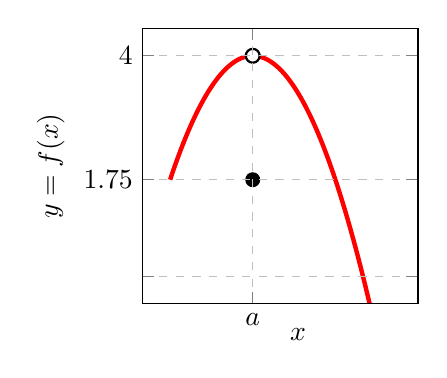
\begin{tikzpicture}[scale=1]
          \begin{axis}[
        %    axis y line = left,
        %    axis x line = bottom,
            xlabel={$x$},
            xtick       = {1.5},
            xticklabels = {$a$},
            ytick       = {0,1.75,4},
            yticklabels = {,$1.75$,$4$},
            samples     = 160,
            domain      = -1:5,
            restrict y to domain=-1:5,
            xmin = -0.5, xmax = 4.5,
            ymin = -0.5, ymax = 4.5,
            grid=both, grid style=dashed,
            width=2in, height=2in,
            y label style={anchor=south},
            ylabel={$y=f(x)$},
        		axis on top,
		x label style={anchor=west},
          ]
          % pieces 1 and 2
          \addplot[domain=0:5, red, ultra thick, mark=none] {4-(x-1.5)^2};
          \filldraw[white] (1.5,4) circle (2.5pt);
          \draw[thick] (1.5,4) circle (2.5pt);
             \filldraw[black] (1.5,1.75) circle (2.5pt);
        \end{axis}
        \end{tikzpicture}
  }{
  \vs{.2}
          \itemI{
		\item As $x$ gets close to $a$ (from the left) the trend of $f(x)$ is towards $4$. \vs{.1}
		\item As $x$ gets close to $a$ (from the right) the trend of $f(x)$ is towards $4$. \vs{.1}
		\item As $x$ gets close to $a$ the trend of $f(x)$ is towards $4$. \vs{.1}
		\item $f(a)=1.75$\vs{.3}
        }
   }{
  \centering {\bf Notation/Observations}
  }
  \vs{-.2}
  \hrule
  ~\\
%  \vs{-.3}
   \mpageTth{.25}{.4}{.35}{
   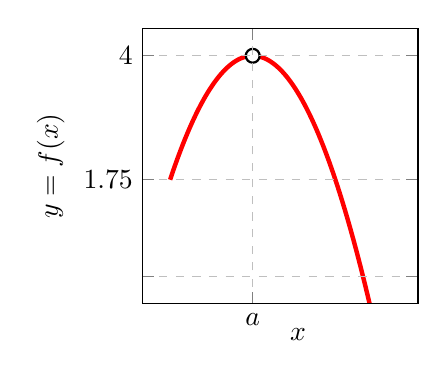
\begin{tikzpicture}[scale=1]
          \begin{axis}[
        %    axis y line = left,
        %    axis x line = bottom,
            xlabel={$x$},
            xtick       = {1.5},
            xticklabels = {$a$},
            ytick       = {0,1.75,4},
            yticklabels = {,$1.75$,$4$},
            samples     = 160,
            domain      = -1:5,
            restrict y to domain=-1:5,
            xmin = -0.5, xmax = 4.5,
            ymin = -0.5, ymax = 4.5,
            grid=both, grid style=dashed,
            width=2in, height=2in,
            y label style={anchor=south},
            ylabel={$y=f(x)$},
        		axis on top,
		x label style={anchor=west},
          ]
          % pieces 1 and 2
          \addplot[domain=0:5, red, ultra thick, mark=none] {4-(x-1.5)^2};
          \filldraw[white] (1.5,4) circle (2.5pt);
          \draw[thick] (1.5,4) circle (2.5pt);
            % \filldraw[black] (1.5,1.75) circle (2.5pt);
        \end{axis}
        \end{tikzpicture}
  }{
\vs{.2} \itemI{
		\item As $x$ gets close to $a$ (from the left) the trend of $f(x)$ is towards $4$. \vs{.1}
		\item As $x$ gets close to $a$ (from the right) the trend of $f(x)$ is towards $4$. \vs{.1}
		\item As $x$ gets close to $a$ the trend of $f(x)$ is towards $4$. \vs{.1}
		\item Ideally, $f(a)=$ \vs{.3}
        }
  }{
  \centering {\bf Notation/Observations}
  }
\vs{-.2}
  \hrule ~\\
\mpageT{.5}{.5}[\hs{.2}]{
\begin{center}{\bf \blue{Informal Key Idea:}} \end{center}
A function is {\em continuous} when you don't have to lift your writing utensil when sketching the graph.
\vs{.25}~\\
{\bf\blue{Why do we care about continuity?}}
\vs{.2}
}{
\begin{center}{\bf \blue{Formal Key Idea:}} \end{center}
A function is {\em continuous} at a number $a$  when 
}
\newpage
\vs{-.5}
\mpageT{.5}{.5}[\hs{.15}]{
\example \ltrm{\color{RoyalBlue}L2} $\ds f(x)=\frac{x^2+1}{x-2}$ is continuous at $x=3$. Find $\ds \lim_{x\to3} \frac{x^2+1}{x-2}$ 
}{
{\exercise }  $\ds f(x)=\frac{\sqrt{x+5}}{x+2}$ is continuous at $x=4$. Find $\ds \lim_{x\to4} \frac{\sqrt{x+5}}{x+2}$.
}
%%%%%%%%%%%%%
\vfill
In the pre-class assignment, you saw the definition of continuity, as well as different types of discontinuities. The goal of this lesson is to learn how to use the definition of continuity to decide whether a function is continuous at a number and to discern between different types of discontinuities.\\

{\bf \textcolor{blue}{Fill in the blanks!}} The pre-class assignment for today's lesson covered the formal {\bf definition of continuity}. 
\begin{center}
{\it The function $f$ is continuous at the number $a$ provided $\displaystyle\lim_{x\to a} f(x)=f(a)$.} \\ % for NTI \unline{.75}{$f(a)$}{.15}
\end{center}

\bigskip

This short definition can be broken up into {\bf three continuity conditions} -- can you remember what they are? The function $f$ is continuous at $a$ provided...  \\

(1) $f(a)$ \unline{1}{}{.15}  \hfill
%
(2) $\displaystyle\lim_{x\to a}f(x)$ \unline{1}{}{.15}\hfill
%
(3) \unline{2}{}{.15} \\[0.3in]

{\bf \blue{Key Question: When is a function {\em not} continuous?}}\\
{\exercise{\color{RoyalBlue} L1}} Given below are graphs of functions discontinuous at $a$:\\

\,\hfill
        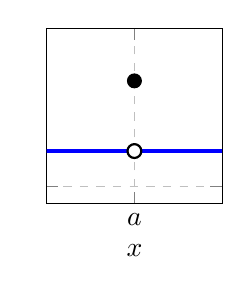
\begin{tikzpicture}[scale=1]
          \begin{axis}[
        %    axis y line = left,
        %    axis x line = bottom,
            xlabel={$x$},
            xtick       = {2},
            xticklabels = {$a$},
            ytick       = {0},
            yticklabels = {},
            samples     = 160,
            domain      = -1:5,
            restrict y to domain=-1:5,
            xmin = -0.5, xmax = 4.5,
            ymin = -0.5, ymax = 4.5,
            grid=both, grid style=dashed,
            width=1.5in, height=1.5in
          ]
          % pieces 1 and 2
          \addplot[domain=-1:5, blue, ultra thick, mark=none] {1};
          \filldraw[white] (2,1) circle (2.5pt);
          \draw[thick] (2,1) circle (2.5pt);
          \filldraw[black] (2,3) circle (2.5pt);
        \end{axis}
        \end{tikzpicture}
        %
        \hfill
        %
        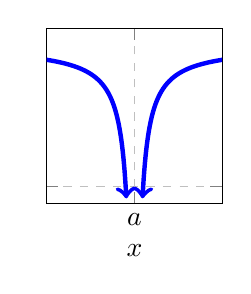
\begin{tikzpicture}[scale=1]
          \begin{axis}[
        %    axis y line = left,
        %    axis x line = bottom,
            xlabel={$x$},
            xtick       = {2},
            xticklabels = {$a$},
            ytick       = {0},
            yticklabels = {},
            samples     = 160,
            domain      = -1:5,
            restrict y to domain=-1:5,
            xmin = -0.5, xmax = 4.5,
            ymin = -0.5, ymax = 4.5,
            grid=both, grid style=dashed,
            width=1.5in, height=1.5in
          ]
          % pieces 1 and 2
          \addplot[domain=-1:1.77, blue, ultra thick, mark=none, <->] {4-abs(x-2)/(x-2)^2};
           \addplot[domain=2.23:5, blue, ultra thick, mark=none, <->] {4-abs(x-2)/(x-2)^2};
        \end{axis}
        \end{tikzpicture}
        %
        \hfill
        %
        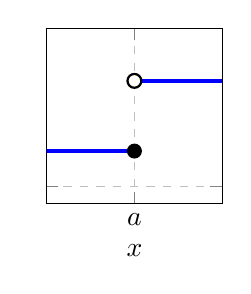
\begin{tikzpicture}[scale=1]
          \begin{axis}[
        %    axis y line = left,
        %    axis x line = bottom,
            xlabel={$x$},
            xtick       = {2},
            xticklabels = {$a$},
            ytick       = {0},
            yticklabels = {},
            samples     = 160,
            domain      = -1:5,
            restrict y to domain=-1:5,
            xmin = -0.5, xmax = 4.5,
            ymin = -0.5, ymax = 4.5,
            grid=both, grid style=dashed,
            width=1.5in, height=1.5in
          ]
          % pieces 1 and 2
          \addplot[domain=-1:2, blue, ultra thick, mark=none] {1};
          \filldraw[black] (2,1) circle (2.5pt);
          \addplot[domain=2:5, blue, ultra thick, mark=none] {3};
          \filldraw[white] (2,3) circle (2.5pt);
          \draw[thick] (2,3) circle (2.5pt);
        \end{axis}
        \end{tikzpicture}
        %
        \hfill
        %
        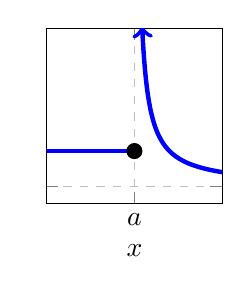
\begin{tikzpicture}[scale=1]
          \begin{axis}[
        %    axis y line = left,
        %    axis x line = bottom,
            xlabel={$x$},
            xtick       = {2},
            xticklabels = {$a$},
            ytick       = {0},
            yticklabels = {},
            samples     = 160,
            domain      = -1:5,
            restrict y to domain=-1:5,
            xmin = -0.5, xmax = 4.5,
            ymin = -0.5, ymax = 4.5,
            grid=both, grid style=dashed,
            width=1.5in, height=1.5in
          ]
          % pieces 1 and 2
          \addplot[domain=-1:2, blue, ultra thick, mark=none] {1};
          \filldraw[black] (2,1) circle (2.5pt);
          \draw[thick] (2,1) circle (2.5pt);
          \addplot[domain=2.22:5, blue, ultra thick, mark=none, <->] {1/(x-2)};
        \end{axis}
        \end{tikzpicture}
        %
        \hfill
        %
        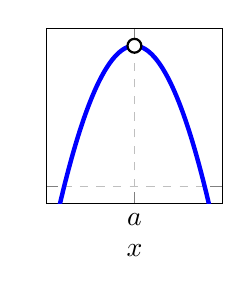
\begin{tikzpicture}[scale=1]
          \begin{axis}[
        %    axis y line = left,
        %    axis x line = bottom,
            xlabel={$x$},
            xtick       = {2},
            xticklabels = {$a$},
            ytick       = {0},
            yticklabels = {},
            samples     = 160,
            domain      = -1:5,
            restrict y to domain=-1:5,
            xmin = -0.5, xmax = 4.5,
            ymin = -0.5, ymax = 4.5,
            grid=both, grid style=dashed,
            width=1.5in, height=1.5in
          ]
          % pieces 1 and 2
          \addplot[domain=-1:5, blue, ultra thick, mark=none] {4-(x-2)^2};
          \filldraw[white] (2,4) circle (2.5pt);
          \draw[thick] (2,4) circle (2.5pt);
        \end{axis}
        \end{tikzpicture}
        %
        \hfill
        %
        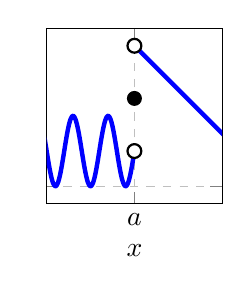
\begin{tikzpicture}[scale=1]
          \begin{axis}[
        %    axis y line = left,
        %    axis x line = bottom,
            xlabel={$x$},
            xtick       = {2},
            xticklabels = {$a$},
            ytick       = {0},
            yticklabels = {},
            samples     = 160,
            domain      = -1:5,
            restrict y to domain=-1:5,
            xmin = -0.5, xmax = 4.5,
            ymin = -0.5, ymax = 4.5,
            grid=both, grid style=dashed,
            width=1.5in, height=1.5in
          ]
          % pieces 1 and 2
          \addplot[domain=-1:2, blue, ultra thick, mark=none] {1+sin(deg(x)*3.141*2)};
          \filldraw[white] (2,1) circle (2.5pt);
          \draw[thick] (2,1) circle (2.5pt);
          \addplot[domain=2:5, blue, ultra thick, mark=none] {6-x};
          \filldraw[white] (2,4) circle (2.5pt);
          \draw[thick] (2,4) circle (2.5pt);
          \filldraw (2,2.5) circle (2.5pt);
        \end{axis}
        \end{tikzpicture}
    \hfill\,\\

\,\hfill 
\unline{.8}{}{.1}
\hfill 
\unline{.8}{}{.1}
\hfill 
\unline{.8}{}{.1}
\hfill 
\unline{.8}{}{.1}
\hfill 
\unline{.8}{}{.1}
\hfill 
\unline{.8}{}{.1}
\hfill\,\\
%
\enumC{
\item[i.] For each graph above, label the graph as depicting a removable, jump, or infinite discontinuity by writing the letters ``RD", ``JD", or ``ID" (respectively) in the blank below the graph.\\
\item[ii.] If a function is discontinuous at a number, then the function must violate at least one of the three conditions you wrote in the fill-in-the-blanks exercise. For each graph above, label the graph with the number(s) of the continuity condition(s) the graph violates in the space below the graph.\\
\item[iii.] Based on your labeling, characterize for each type of discontinuity which continuity conditions must be satisfied or violated.

\itemC{
\item $f$ has a {\bf removable} discontinuity at $a$ {\it always} means:\\\\
\item $f$ has a {\bf jump} discontinuity at $a$ {\it always} means:\\\\
\item $f$ has an {\bf infinite} discontinuity at $a$ {\it always} means:\\\\
}

}

%%%%%%%%%
\newpage%
%%%%%%%%%

{\bf\color{blue}When can we be confident that a function {\em is} continuous?} The pre-class assignment for today's lesson covered the Main Continuity Theorem and the Rules for Finding Domains:
%
\important{The Main Continuity Theorem}
{
%
\,\\[-0.05in]
%
Any function that is some combination \\  of other continuous functions\\
 (polynomials, \hfill roots, \hfill   trigonometric functions, \hfill exponentials, logarithms, \hfil or absolute value)
\vs{.3}\\
is continuous on its \unline{1}{}{.15}.
%
}

 {\bf \blue{Practical Rules for determining when a number is {\em not} in a domain}}\\
 A number is {\em not} in the domain when one of the following situations occur:
 % problems Therefore, determining where familiar functions are continuous involves finding the domain of those functions, so let's record the rules for finding domains.
\vspace{10cm}

\example{\color{RoyalBlue}L2}/ \exercise{\color{RoyalBlue}L2} For each of the following limits, decide whether the Main Continuity Theorem applies. If the theorem applies, then find the limit. If the theorem does not apply, then explain why.

\tasksA{2}{
\task ({\bf\color{blue}Example}) $\displaystyle\lim_{x\to-1}\dfrac{x+1}{x-1}$ 
\task ({\bf\color{blue}Example}) $\displaystyle\lim_{x\to1}\dfrac{1}{\sqrt{x-1}}$ 
\newpage
\vs{1.6}
\task ({\bf\color{blue}Exercise}) $\displaystyle\lim_{x\to3}\dfrac{x^3+1}{x-3}$
\task ({\bf\color{blue}Exercise}) $\displaystyle\lim_{x\to0}\dfrac{1}{\sqrt{x-1}}$ 
\vs{2.2}
\task ({\bf\color{blue}Exercise}) $\displaystyle\lim_{x\to4}\dfrac{\sqrt{x^2-4}+1}{x-7}$
}
\vs{2.2}
%\hfill {\small\it(parts (f) and (g) are on the next page $\to$)}
%\newpage
\tasksAS{2}{6}{
\task ({\bf\color{blue}Extra Practice}) $\displaystyle\lim_{x\to0}\dfrac{x-2}{e^x-1}$
\task ({\bf\color{blue}Extra Practice}) $\displaystyle\lim_{x\to2}\dfrac{x-2}{e^x-1}$
}

\newpage

\example{\color{RoyalBlue}L1} Some very powerful mathematics we will learn later this semester depends upon being able to identify whether a function is continuous on an interval of $x$-values. Let's practice that skill here!\\

On which of the following intervals is $f(x)=\dfrac{\ln(x)}{x-4}$ continuous? Circle all that apply, and explain below.
\tasksA{4}{
\task  $[5,8]$ 
\task $[0,2]$ 
\task $[1,5]$ 
\task $[-7,-1]$ 
}
\vfill
\exercise{\color{RoyalBlue}L1} Give 1 example of an interval on which $g(x)=\dfrac{1}{\sqrt{x-1}}$ {\em is} continuous, and 1 example of an interval where $g$  {\em is not} continuous.   Explain why your examples are correct.
\vfill


%\hrulefill\\

\newpage
The following problem appeared first during the Spring 2023 semester. Note that you must know the 3 continuity conditions and how to interpret them graphically to successfully address the prompt!\\

{\bf\color{blue} Exam Practice 1.}{\reversemarginpar\marginnote{\fbox{\bf\color{RoyalBlue}L1}}} On each set of axes below, draw an example of a function that satisfies the condition written.
\tasksA{4}{
%
\task \\ \begin{minipage}[t]{0.22\textwidth}
    \begin{center}
    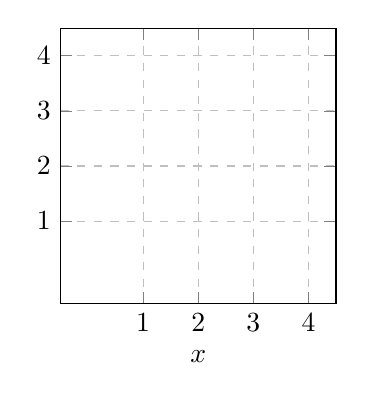
\begin{tikzpicture}[scale=1]
          \begin{axis}[
        %    axis y line = left,
        %    axis x line = bottom,
            xlabel={$x$},
            xtick       = {1,2,3,4},
            xticklabels = {1,2,3,4},
            ytick       = {1,2,3,4},
            yticklabels = {1,2,3,4},
            samples     = 160,
            domain      = -1:5,
            restrict y to domain=-1:5,
            xmin = -0.5, xmax = 4.5,
            ymin = -0.5, ymax = 4.5,
            grid=both, grid style=dashed,
            width=2in, height=2in
          ]
        \end{axis}
    \end{tikzpicture}
    continuous at $2$
    \end{center}
\end{minipage}
%

%
\task \\ \begin{minipage}[t]{0.22\textwidth}
    \begin{center}
    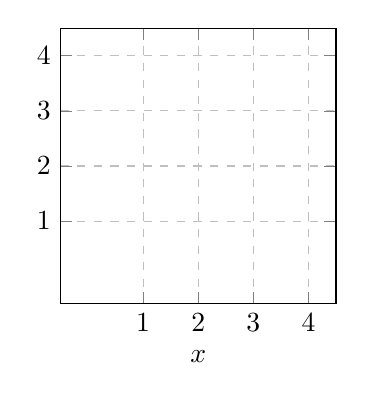
\begin{tikzpicture}[scale=1]
          \begin{axis}[
        %    axis y line = left,
        %    axis x line = bottom,
            xlabel={$x$},
            xtick       = {1,2,3,4},
            xticklabels = {1,2,3,4},
            ytick       = {1,2,3,4},
            yticklabels = {1,2,3,4},
            samples     = 160,
            domain      = -1:5,
            restrict y to domain=-1:5,
            xmin = -0.5, xmax = 4.5,
            ymin = -0.5, ymax = 4.5,
            grid=both, grid style=dashed,
            width=2in, height=2in
          ]
        \end{axis}
    \end{tikzpicture}
    discontinuous at $2$ because only continuity conditions (1) \& (3) fail
    \end{center}
\end{minipage}
%

%
\task \\ \begin{minipage}[t]{0.22\textwidth}
    \begin{center}
    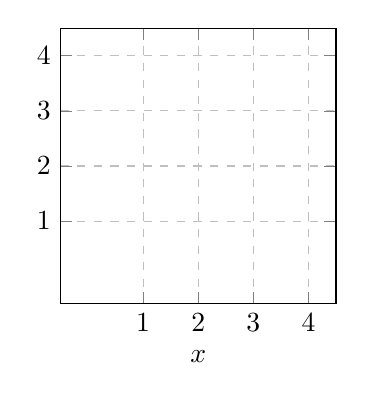
\begin{tikzpicture}[scale=1]
          \begin{axis}[
        %    axis y line = left,
        %    axis x line = bottom,
            xlabel={$x$},
            xtick       = {1,2,3,4},
            xticklabels = {1,2,3,4},
            ytick       = {1,2,3,4},
            yticklabels = {1,2,3,4},
            samples     = 160,
            domain      = -1:5,
            restrict y to domain=-1:5,
            xmin = -0.5, xmax = 4.5,
            ymin = -0.5, ymax = 4.5,
            grid=both, grid style=dashed,
            width=2in, height=2in
          ]
        \end{axis}
    \end{tikzpicture}
    discontinuous at $2$ because only continuity conditions (2) \& (3) fail
    \end{center}
\end{minipage}
%

%
\task \\ \begin{minipage}[t]{0.22\textwidth}
\begin{center}
    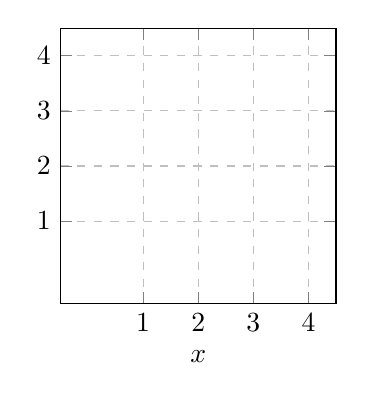
\begin{tikzpicture}[scale=1]
          \begin{axis}[
        %    axis y line = left,
        %    axis x line = bottom,
            xlabel={$x$},
            xtick       = {1,2,3,4},
            xticklabels = {1,2,3,4},
            ytick       = {1,2,3,4},
            yticklabels = {1,2,3,4},
            samples     = 160,
            domain      = -1:5,
            restrict y to domain=-1:5,
            xmin = -0.5, xmax = 4.5,
            ymin = -0.5, ymax = 4.5,
            grid=both, grid style=dashed,
            width=2in, height=2in
          ]
        \end{axis}
    \end{tikzpicture}
    discontinuous at $2$ because only continuity condition (3) fails
    \end{center}
\end{minipage}
}

\end{document}